\documentclass[]{article}
\usepackage{lmodern}
\usepackage{amssymb,amsmath}
\usepackage{ifxetex,ifluatex}
\usepackage{fixltx2e} % provides \textsubscript
\ifnum 0\ifxetex 1\fi\ifluatex 1\fi=0 % if pdftex
  \usepackage[T1]{fontenc}
  \usepackage[utf8]{inputenc}
\else % if luatex or xelatex
  \ifxetex
    \usepackage{mathspec}
  \else
    \usepackage{fontspec}
  \fi
  \defaultfontfeatures{Ligatures=TeX,Scale=MatchLowercase}
\fi
% use upquote if available, for straight quotes in verbatim environments
\IfFileExists{upquote.sty}{\usepackage{upquote}}{}
% use microtype if available
\IfFileExists{microtype.sty}{%
\usepackage{microtype}
\UseMicrotypeSet[protrusion]{basicmath} % disable protrusion for tt fonts
}{}
\usepackage[margin=1in]{geometry}
\usepackage{hyperref}
\hypersetup{unicode=true,
            pdftitle={StateCoronavirusAnalysis},
            pdfauthor={Stephen R. Proulx},
            pdfborder={0 0 0},
            breaklinks=true}
\urlstyle{same}  % don't use monospace font for urls
\usepackage{color}
\usepackage{fancyvrb}
\newcommand{\VerbBar}{|}
\newcommand{\VERB}{\Verb[commandchars=\\\{\}]}
\DefineVerbatimEnvironment{Highlighting}{Verbatim}{commandchars=\\\{\}}
% Add ',fontsize=\small' for more characters per line
\usepackage{framed}
\definecolor{shadecolor}{RGB}{248,248,248}
\newenvironment{Shaded}{\begin{snugshade}}{\end{snugshade}}
\newcommand{\AlertTok}[1]{\textcolor[rgb]{0.94,0.16,0.16}{#1}}
\newcommand{\AnnotationTok}[1]{\textcolor[rgb]{0.56,0.35,0.01}{\textbf{\textit{#1}}}}
\newcommand{\AttributeTok}[1]{\textcolor[rgb]{0.77,0.63,0.00}{#1}}
\newcommand{\BaseNTok}[1]{\textcolor[rgb]{0.00,0.00,0.81}{#1}}
\newcommand{\BuiltInTok}[1]{#1}
\newcommand{\CharTok}[1]{\textcolor[rgb]{0.31,0.60,0.02}{#1}}
\newcommand{\CommentTok}[1]{\textcolor[rgb]{0.56,0.35,0.01}{\textit{#1}}}
\newcommand{\CommentVarTok}[1]{\textcolor[rgb]{0.56,0.35,0.01}{\textbf{\textit{#1}}}}
\newcommand{\ConstantTok}[1]{\textcolor[rgb]{0.00,0.00,0.00}{#1}}
\newcommand{\ControlFlowTok}[1]{\textcolor[rgb]{0.13,0.29,0.53}{\textbf{#1}}}
\newcommand{\DataTypeTok}[1]{\textcolor[rgb]{0.13,0.29,0.53}{#1}}
\newcommand{\DecValTok}[1]{\textcolor[rgb]{0.00,0.00,0.81}{#1}}
\newcommand{\DocumentationTok}[1]{\textcolor[rgb]{0.56,0.35,0.01}{\textbf{\textit{#1}}}}
\newcommand{\ErrorTok}[1]{\textcolor[rgb]{0.64,0.00,0.00}{\textbf{#1}}}
\newcommand{\ExtensionTok}[1]{#1}
\newcommand{\FloatTok}[1]{\textcolor[rgb]{0.00,0.00,0.81}{#1}}
\newcommand{\FunctionTok}[1]{\textcolor[rgb]{0.00,0.00,0.00}{#1}}
\newcommand{\ImportTok}[1]{#1}
\newcommand{\InformationTok}[1]{\textcolor[rgb]{0.56,0.35,0.01}{\textbf{\textit{#1}}}}
\newcommand{\KeywordTok}[1]{\textcolor[rgb]{0.13,0.29,0.53}{\textbf{#1}}}
\newcommand{\NormalTok}[1]{#1}
\newcommand{\OperatorTok}[1]{\textcolor[rgb]{0.81,0.36,0.00}{\textbf{#1}}}
\newcommand{\OtherTok}[1]{\textcolor[rgb]{0.56,0.35,0.01}{#1}}
\newcommand{\PreprocessorTok}[1]{\textcolor[rgb]{0.56,0.35,0.01}{\textit{#1}}}
\newcommand{\RegionMarkerTok}[1]{#1}
\newcommand{\SpecialCharTok}[1]{\textcolor[rgb]{0.00,0.00,0.00}{#1}}
\newcommand{\SpecialStringTok}[1]{\textcolor[rgb]{0.31,0.60,0.02}{#1}}
\newcommand{\StringTok}[1]{\textcolor[rgb]{0.31,0.60,0.02}{#1}}
\newcommand{\VariableTok}[1]{\textcolor[rgb]{0.00,0.00,0.00}{#1}}
\newcommand{\VerbatimStringTok}[1]{\textcolor[rgb]{0.31,0.60,0.02}{#1}}
\newcommand{\WarningTok}[1]{\textcolor[rgb]{0.56,0.35,0.01}{\textbf{\textit{#1}}}}
\usepackage{graphicx,grffile}
\makeatletter
\def\maxwidth{\ifdim\Gin@nat@width>\linewidth\linewidth\else\Gin@nat@width\fi}
\def\maxheight{\ifdim\Gin@nat@height>\textheight\textheight\else\Gin@nat@height\fi}
\makeatother
% Scale images if necessary, so that they will not overflow the page
% margins by default, and it is still possible to overwrite the defaults
% using explicit options in \includegraphics[width, height, ...]{}
\setkeys{Gin}{width=\maxwidth,height=\maxheight,keepaspectratio}
\IfFileExists{parskip.sty}{%
\usepackage{parskip}
}{% else
\setlength{\parindent}{0pt}
\setlength{\parskip}{6pt plus 2pt minus 1pt}
}
\setlength{\emergencystretch}{3em}  % prevent overfull lines
\providecommand{\tightlist}{%
  \setlength{\itemsep}{0pt}\setlength{\parskip}{0pt}}
\setcounter{secnumdepth}{0}
% Redefines (sub)paragraphs to behave more like sections
\ifx\paragraph\undefined\else
\let\oldparagraph\paragraph
\renewcommand{\paragraph}[1]{\oldparagraph{#1}\mbox{}}
\fi
\ifx\subparagraph\undefined\else
\let\oldsubparagraph\subparagraph
\renewcommand{\subparagraph}[1]{\oldsubparagraph{#1}\mbox{}}
\fi

%%% Use protect on footnotes to avoid problems with footnotes in titles
\let\rmarkdownfootnote\footnote%
\def\footnote{\protect\rmarkdownfootnote}

%%% Change title format to be more compact
\usepackage{titling}

% Create subtitle command for use in maketitle
\providecommand{\subtitle}[1]{
  \posttitle{
    \begin{center}\large#1\end{center}
    }
}

\setlength{\droptitle}{-2em}

  \title{StateCoronavirusAnalysis}
    \pretitle{\vspace{\droptitle}\centering\huge}
  \posttitle{\par}
    \author{Stephen R. Proulx}
    \preauthor{\centering\large\emph}
  \postauthor{\par}
      \predate{\centering\large\emph}
  \postdate{\par}
    \date{3/14/2020}


\begin{document}
\maketitle

\#\#Gather and process the data

\begin{Shaded}
\begin{Highlighting}[]
\NormalTok{confirmed_sheet<-}\KeywordTok{read.csv}\NormalTok{(}\StringTok{"https://raw.githubusercontent.com/CSSEGISandData/COVID-19/master/csse_covid_19_data/csse_covid_19_time_series/time_series_19-covid-Confirmed.csv"}\NormalTok{) }\OperatorTok
\StringTok{  }\KeywordTok{select}\NormalTok{(}\OperatorTok{-}\NormalTok{Lat, }\OperatorTok{-}\NormalTok{Long)}
\NormalTok{deaths_sheet <-}\StringTok{ }\KeywordTok{read.csv}\NormalTok{(}\StringTok{"https://raw.githubusercontent.com/CSSEGISandData/COVID-19/master/csse_covid_19_data/csse_covid_19_time_series/time_series_19-covid-Deaths.csv"}\NormalTok{)}\OperatorTok
\StringTok{  }\KeywordTok{select}\NormalTok{(}\OperatorTok{-}\NormalTok{Lat, }\OperatorTok{-}\NormalTok{Long)}
\NormalTok{recovered_sheet <-}\StringTok{ }\KeywordTok{read.csv}\NormalTok{(}\StringTok{"https://raw.githubusercontent.com/CSSEGISandData/COVID-19/master/csse_covid_19_data/csse_covid_19_time_series/time_series_19-covid-Recovered.csv"}\NormalTok{)}\OperatorTok
\StringTok{  }\KeywordTok{select}\NormalTok{(}\OperatorTok{-}\NormalTok{Lat, }\OperatorTok{-}\NormalTok{Long) }



\NormalTok{confirmed_long <-}\StringTok{ }\KeywordTok{gather}\NormalTok{(confirmed_sheet, }\OperatorTok{-}\NormalTok{Province.State , }\OperatorTok{-}\NormalTok{Country.Region , }\DataTypeTok{key=}\StringTok{"date"}\NormalTok{, }\DataTypeTok{value =} \StringTok{"cases"}\NormalTok{)}\OperatorTok
\StringTok{  }\KeywordTok{separate}\NormalTok{(date,}\KeywordTok{c}\NormalTok{(}\StringTok{"x"}\NormalTok{,}\StringTok{"date.longer"}\NormalTok{),}\DecValTok{1}\NormalTok{,}\DataTypeTok{remove=}\OtherTok{TRUE}\NormalTok{) }\OperatorTok\StringTok{ }
\StringTok{  }\KeywordTok{separate}\NormalTok{(date.longer,}\KeywordTok{c}\NormalTok{(}\StringTok{"month"}\NormalTok{,}\StringTok{"day"}\NormalTok{,}\StringTok{"year"}\NormalTok{),}\DataTypeTok{remove=}\OtherTok{TRUE}\NormalTok{) }\OperatorTok
\StringTok{  }\KeywordTok{separate}\NormalTok{(Province.State,}\KeywordTok{c}\NormalTok{(}\StringTok{"location"}\NormalTok{,}\StringTok{"State"}\NormalTok{),}\DataTypeTok{sep=}\StringTok{", "}\NormalTok{,}\DataTypeTok{remove=}\OtherTok{FALSE}\NormalTok{) }\OperatorTok\StringTok{ }\CommentTok{#for US data before 3/10/2020 Province.State value includes sub-state location data. Split this out so that we can recover state level data later.}
\StringTok{  }\KeywordTok{mutate}\NormalTok{(}\DataTypeTok{location =} \KeywordTok{as.character}\NormalTok{(location)) }\OperatorTok
\StringTok{  }\KeywordTok{mutate}\NormalTok{(}\DataTypeTok{State =} \KeywordTok{as.character}\NormalTok{(State)) }\OperatorTok
\StringTok{  }\KeywordTok{mutate}\NormalTok{(}\DataTypeTok{year=}\KeywordTok{as.character}\NormalTok{(}\KeywordTok{as.numeric}\NormalTok{(year)}\OperatorTok{+}\DecValTok{2000}\NormalTok{)) }\OperatorTok\StringTok{ }\CommentTok{#data was in a format with just the last two digits for year}
\StringTok{  }\KeywordTok{unite}\NormalTok{(comb.date, }\KeywordTok{c}\NormalTok{(month,day,year) , }\DataTypeTok{sep=}\StringTok{"."}\NormalTok{)}\OperatorTok\StringTok{  }
\StringTok{  }\KeywordTok{mutate}\NormalTok{(}\DataTypeTok{date =} \KeywordTok{parse_date}\NormalTok{(comb.date , }\StringTok{"%m%.%d%.%Y"}\NormalTok{))}\OperatorTok
\StringTok{  }\KeywordTok{select}\NormalTok{(}\OperatorTok{-}\NormalTok{comb.date , }\OperatorTok{-}\NormalTok{x) }\OperatorTok
\StringTok{  }\KeywordTok{mutate}\NormalTok{(}\DataTypeTok{delta.days=}\KeywordTok{period_to_seconds}\NormalTok{(}\KeywordTok{days}\NormalTok{(}\KeywordTok{ymd}\NormalTok{(date) }\OperatorTok{-}\StringTok{ }\KeywordTok{ymd}\NormalTok{(}\DecValTok{20200122}\NormalTok{)))}\OperatorTok{/}\NormalTok{(}\DecValTok{60}\OperatorTok{*}\DecValTok{60}\OperatorTok{*}\DecValTok{24}\NormalTok{)) }\OperatorTok\StringTok{ }\CommentTok{#calculate days since data began being collected}
\StringTok{  }\KeywordTok{as_tibble}\NormalTok{()  }
\end{Highlighting}
\end{Shaded}

\begin{verbatim}
## Warning: Expected 2 pieces. Missing pieces filled with `NA` in 14960
## rows [1, 2, 3, 4, 5, 6, 7, 8, 9, 10, 11, 12, 13, 14, 15, 16, 17, 18, 19,
## 20, ...].
\end{verbatim}

Unfortunately the data seems to be grouped into locations that are not
consistent throughout the dataset. Before March 10, 2020, the US data is
presented by city or county within each state, but after March 10 it is
aggregated by state.

For data befor March 10, go through each state to process and combine
the data from the different locations.

\begin{Shaded}
\begin{Highlighting}[]
\NormalTok{wash.data.substate <-}\StringTok{ }\KeywordTok{filter}\NormalTok{(confirmed_long,Country.Region}\OperatorTok{==}\StringTok{"US"}\NormalTok{ ,State}\OperatorTok{==}\StringTok{"WA"}\NormalTok{) }\OperatorTok\StringTok{  }
\StringTok{  }\KeywordTok{filter}\NormalTok{(delta.days}\OperatorTok{<}\DecValTok{48}\NormalTok{) }\OperatorTok
\StringTok{  }\KeywordTok{group_by}\NormalTok{(date,State, delta.days, Country.Region) }\OperatorTok\StringTok{ }\KeywordTok{summarise}\NormalTok{(}\DataTypeTok{mean=}\KeywordTok{mean}\NormalTok{(cases), }\DataTypeTok{count=}\KeywordTok{n}\NormalTok{() ) }\OperatorTok
\StringTok{  }\KeywordTok{mutate}\NormalTok{(}\DataTypeTok{total.cases =}\NormalTok{ mean}\OperatorTok{*}\NormalTok{count) }\OperatorTok\StringTok{ }
\StringTok{  }\KeywordTok{select}\NormalTok{(}\OperatorTok{-}\NormalTok{mean, }\OperatorTok{-}\NormalTok{count)  }


\NormalTok{wash.data.state <-}\StringTok{ }\KeywordTok{filter}\NormalTok{(confirmed_long,Country.Region}\OperatorTok{==}\StringTok{"US"}\NormalTok{ , Province.State}\OperatorTok{==}\StringTok{"Washington"}\NormalTok{) }\OperatorTok\StringTok{ }
\StringTok{  }\KeywordTok{filter}\NormalTok{(delta.days}\OperatorTok{>}\DecValTok{47}\NormalTok{) }\OperatorTok
\StringTok{  }\KeywordTok{mutate}\NormalTok{(}\DataTypeTok{State =} \StringTok{"WA"}\NormalTok{ , }\DataTypeTok{total.cases=}\NormalTok{cases) }\OperatorTok
\StringTok{  }\KeywordTok{select}\NormalTok{(}\OperatorTok{-}\NormalTok{Province.State,}\OperatorTok{-}\NormalTok{location,}\OperatorTok{-}\NormalTok{cases)}


\NormalTok{WA.data.state <-}\StringTok{ }\KeywordTok{bind_rows}\NormalTok{(wash.data.state,wash.data.substate) }
\end{Highlighting}
\end{Shaded}

\begin{Shaded}
\begin{Highlighting}[]
\NormalTok{CA.data.substate <-}\StringTok{ }\KeywordTok{filter}\NormalTok{(confirmed_long,Country.Region}\OperatorTok{==}\StringTok{"US"}\NormalTok{ ,State}\OperatorTok{==}\StringTok{"CA"}\NormalTok{, Province.State}\OperatorTok{!=}\StringTok{"Diamond Princess"}\NormalTok{,Province.State}\OperatorTok{!=}\StringTok{"Grand Princess"}\NormalTok{) }\OperatorTok\StringTok{  }
\StringTok{  }\KeywordTok{filter}\NormalTok{(delta.days}\OperatorTok{<}\DecValTok{48}\NormalTok{) }\OperatorTok
\StringTok{  }\KeywordTok{group_by}\NormalTok{(date,State, delta.days, Country.Region) }\OperatorTok\StringTok{ }\KeywordTok{summarise}\NormalTok{(}\DataTypeTok{mean=}\KeywordTok{mean}\NormalTok{(cases), }\DataTypeTok{count=}\KeywordTok{n}\NormalTok{() ) }\OperatorTok
\StringTok{  }\KeywordTok{mutate}\NormalTok{(}\DataTypeTok{total.cases =}\NormalTok{ mean}\OperatorTok{*}\NormalTok{count) }\OperatorTok\StringTok{ }
\StringTok{  }\KeywordTok{select}\NormalTok{(}\OperatorTok{-}\NormalTok{mean, }\OperatorTok{-}\NormalTok{count)  }


\NormalTok{CA.data.state <-}\StringTok{ }\KeywordTok{filter}\NormalTok{(confirmed_long,Country.Region}\OperatorTok{==}\StringTok{"US"}\NormalTok{ , Province.State}\OperatorTok{==}\StringTok{"California"}\NormalTok{) }\OperatorTok\StringTok{ }
\StringTok{  }\KeywordTok{filter}\NormalTok{(delta.days}\OperatorTok{>}\DecValTok{47}\NormalTok{) }\OperatorTok
\StringTok{  }\KeywordTok{mutate}\NormalTok{(}\DataTypeTok{State =} \StringTok{"CA"}\NormalTok{ , }\DataTypeTok{total.cases=}\NormalTok{cases) }\OperatorTok
\StringTok{  }\KeywordTok{select}\NormalTok{(}\OperatorTok{-}\NormalTok{Province.State,}\OperatorTok{-}\NormalTok{location,}\OperatorTok{-}\NormalTok{cases)}


\NormalTok{CA.data.state <-}\StringTok{ }\KeywordTok{bind_rows}\NormalTok{(CA.data.state,CA.data.substate)  }
\end{Highlighting}
\end{Shaded}

\begin{Shaded}
\begin{Highlighting}[]
\NormalTok{NY.data.substate <-}\StringTok{ }\KeywordTok{filter}\NormalTok{(confirmed_long,Country.Region}\OperatorTok{==}\StringTok{"US"}\NormalTok{ ,State}\OperatorTok{==}\StringTok{"NY"}\NormalTok{) }\OperatorTok\StringTok{  }
\StringTok{  }\KeywordTok{filter}\NormalTok{(delta.days}\OperatorTok{<}\DecValTok{48}\NormalTok{) }\OperatorTok
\StringTok{  }\KeywordTok{group_by}\NormalTok{(date,State, delta.days, Country.Region) }\OperatorTok\StringTok{ }\KeywordTok{summarise}\NormalTok{(}\DataTypeTok{mean=}\KeywordTok{mean}\NormalTok{(cases), }\DataTypeTok{count=}\KeywordTok{n}\NormalTok{() ) }\OperatorTok
\StringTok{  }\KeywordTok{mutate}\NormalTok{(}\DataTypeTok{total.cases =}\NormalTok{ mean}\OperatorTok{*}\NormalTok{count) }\OperatorTok\StringTok{ }
\StringTok{  }\KeywordTok{select}\NormalTok{(}\OperatorTok{-}\NormalTok{mean, }\OperatorTok{-}\NormalTok{count)  }

\NormalTok{NY.data.state <-}\StringTok{ }\KeywordTok{filter}\NormalTok{(confirmed_long,Country.Region}\OperatorTok{==}\StringTok{"US"}\NormalTok{ , Province.State}\OperatorTok{==}\StringTok{"New York"}\NormalTok{) }\OperatorTok\StringTok{ }
\StringTok{  }\KeywordTok{filter}\NormalTok{(delta.days}\OperatorTok{>}\DecValTok{47}\NormalTok{) }\OperatorTok
\StringTok{  }\KeywordTok{mutate}\NormalTok{(}\DataTypeTok{State =} \StringTok{"NY"}\NormalTok{ , }\DataTypeTok{total.cases=}\NormalTok{cases) }\OperatorTok
\StringTok{  }\KeywordTok{select}\NormalTok{(}\OperatorTok{-}\NormalTok{Province.State,}\OperatorTok{-}\NormalTok{location,}\OperatorTok{-}\NormalTok{cases)}


\NormalTok{NY.data.state <-}\StringTok{ }\KeywordTok{bind_rows}\NormalTok{(NY.data.state,NY.data.substate)  }
\end{Highlighting}
\end{Shaded}

\begin{Shaded}
\begin{Highlighting}[]
\NormalTok{MA.data.substate <-}\StringTok{ }\KeywordTok{filter}\NormalTok{(confirmed_long,Country.Region}\OperatorTok{==}\StringTok{"US"}\NormalTok{ ,State}\OperatorTok{==}\StringTok{"MA"}\NormalTok{) }\OperatorTok\StringTok{  }
\StringTok{  }\KeywordTok{filter}\NormalTok{(delta.days}\OperatorTok{<}\DecValTok{48}\NormalTok{) }\OperatorTok
\StringTok{  }\KeywordTok{group_by}\NormalTok{(date,State, delta.days, Country.Region) }\OperatorTok\StringTok{ }\KeywordTok{summarise}\NormalTok{(}\DataTypeTok{mean=}\KeywordTok{mean}\NormalTok{(cases), }\DataTypeTok{count=}\KeywordTok{n}\NormalTok{() ) }\OperatorTok
\StringTok{  }\KeywordTok{mutate}\NormalTok{(}\DataTypeTok{total.cases =}\NormalTok{ mean}\OperatorTok{*}\NormalTok{count) }\OperatorTok\StringTok{ }
\StringTok{  }\KeywordTok{select}\NormalTok{(}\OperatorTok{-}\NormalTok{mean, }\OperatorTok{-}\NormalTok{count)  }

\NormalTok{MA.data.state <-}\StringTok{ }\KeywordTok{filter}\NormalTok{(confirmed_long,Country.Region}\OperatorTok{==}\StringTok{"US"}\NormalTok{ , Province.State}\OperatorTok{==}\StringTok{"Massachusetts"}\NormalTok{) }\OperatorTok\StringTok{ }
\StringTok{  }\KeywordTok{filter}\NormalTok{(delta.days}\OperatorTok{>}\DecValTok{47}\NormalTok{) }\OperatorTok
\StringTok{  }\KeywordTok{mutate}\NormalTok{(}\DataTypeTok{State =} \StringTok{"MA"}\NormalTok{ , }\DataTypeTok{total.cases=}\NormalTok{cases) }\OperatorTok
\StringTok{  }\KeywordTok{select}\NormalTok{(}\OperatorTok{-}\NormalTok{Province.State,}\OperatorTok{-}\NormalTok{location,}\OperatorTok{-}\NormalTok{cases)}


\NormalTok{MA.data.state <-}\StringTok{ }\KeywordTok{bind_rows}\NormalTok{(MA.data.state,MA.data.substate)  }
\end{Highlighting}
\end{Shaded}

\#\#\#Plot the stae specific data

\begin{Shaded}
\begin{Highlighting}[]
\NormalTok{State.Totals <-}\StringTok{ }\KeywordTok{bind_rows}\NormalTok{(MA.data.state,WA.data.state,CA.data.state,NY.data.state) }\OperatorTok\StringTok{ }\KeywordTok{mutate}\NormalTok{(}\DataTypeTok{wday=}\KeywordTok{wday}\NormalTok{(date,}\DataTypeTok{label=}\OtherTok{TRUE}\NormalTok{))}


\KeywordTok{ggplot}\NormalTok{(}\DataTypeTok{data=}\KeywordTok{filter}\NormalTok{(State.Totals,total.cases}\OperatorTok{>}\DecValTok{20}\NormalTok{) , }\KeywordTok{aes}\NormalTok{(}\DataTypeTok{x=}\NormalTok{delta.days,}\DataTypeTok{y=}\KeywordTok{log}\NormalTok{(total.cases, }\DataTypeTok{base=}\DecValTok{10}\NormalTok{) ,}\DataTypeTok{color=}\NormalTok{State,  }\DataTypeTok{group=}\NormalTok{State)) }\OperatorTok{+}
\StringTok{  }\KeywordTok{geom_point}\NormalTok{()}\OperatorTok{+}
\StringTok{    }\KeywordTok{geom_smooth}\NormalTok{( }\DataTypeTok{method =} \StringTok{"lm"}\NormalTok{ )}\OperatorTok{+}\StringTok{  }
\StringTok{  }\KeywordTok{scale_y_continuous}\NormalTok{( }\DataTypeTok{limits=}\KeywordTok{c}\NormalTok{(}\DecValTok{1}\NormalTok{,}\FloatTok{3.5}\NormalTok{),}\DataTypeTok{breaks=}\KeywordTok{c}\NormalTok{(}\DecValTok{1}\NormalTok{,}\DecValTok{2}\NormalTok{,}\DecValTok{3}\NormalTok{), }\DataTypeTok{labels=}\KeywordTok{c}\NormalTok{(}\DecValTok{10}\NormalTok{,}\DecValTok{100}\NormalTok{,}\DecValTok{1000}\NormalTok{))}\OperatorTok{+}
\StringTok{  }\KeywordTok{labs}\NormalTok{( }\DataTypeTok{x=}\StringTok{"days since Jan 22"}\NormalTok{ , }\DataTypeTok{y=}\StringTok{"cases per state"}\NormalTok{)}
\end{Highlighting}
\end{Shaded}

\begin{verbatim}
## `geom_smooth()` using formula 'y ~ x'
\end{verbatim}

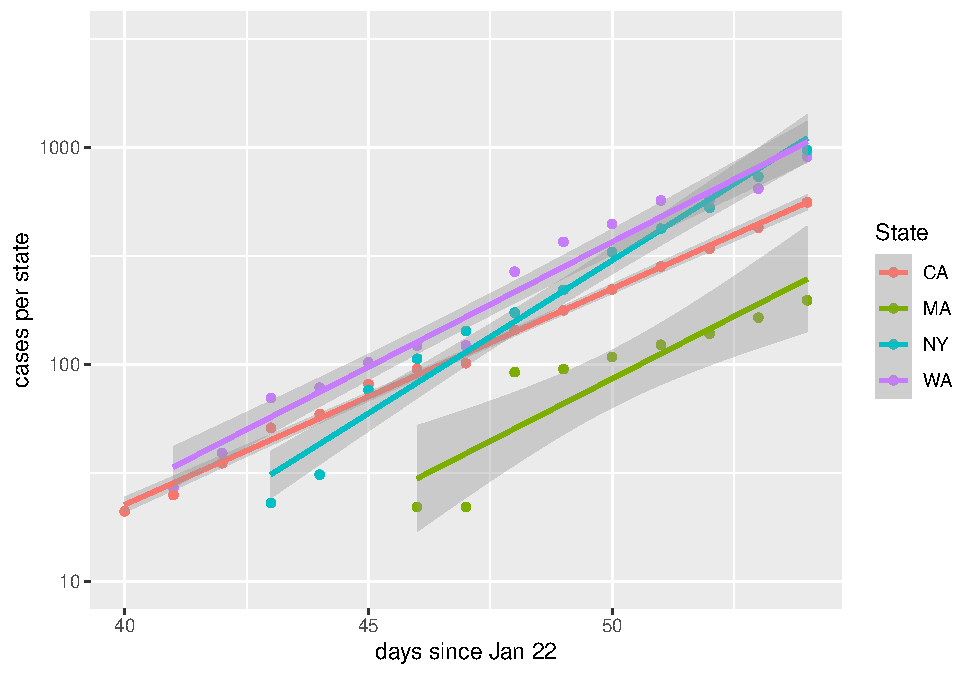
\includegraphics{PlotData_files/figure-latex/combineStateTotals-1.pdf}

\#\#\#Plot the country specific data

The US and China data are split by within-country region, so we must sum
up the Province.State entries to get the total. The new tibble
confirmed\_long2 has the non-aggregated US and China data removed and
has them replaced by the aggregated version.

\begin{Shaded}
\begin{Highlighting}[]
\NormalTok{USTotals <-}\StringTok{ }\KeywordTok{filter}\NormalTok{(confirmed_long,Country.Region}\OperatorTok{==}\StringTok{"US"}\NormalTok{ ) }\OperatorTok\StringTok{  }
\StringTok{  }\KeywordTok{group_by}\NormalTok{(date, delta.days, Country.Region) }\OperatorTok\StringTok{ }\KeywordTok{summarise}\NormalTok{(}\DataTypeTok{mean=}\KeywordTok{mean}\NormalTok{(cases), }\DataTypeTok{count=}\KeywordTok{n}\NormalTok{() ) }\OperatorTok
\StringTok{  }\KeywordTok{mutate}\NormalTok{(}\DataTypeTok{total.cases =}\NormalTok{ mean}\OperatorTok{*}\NormalTok{count) }\OperatorTok\StringTok{ }
\StringTok{  }\KeywordTok{select}\NormalTok{(}\OperatorTok{-}\NormalTok{mean, }\OperatorTok{-}\NormalTok{count)  }\OperatorTok
\CommentTok{#  mutate(Country.Region = "USA") %>%}
\StringTok{  }\KeywordTok{rename}\NormalTok{(}\DataTypeTok{cases=}\NormalTok{total.cases) }

\NormalTok{ChinaTotals <-}\StringTok{ }\KeywordTok{filter}\NormalTok{(confirmed_long,Country.Region}\OperatorTok{==}\StringTok{"China"}\NormalTok{ ) }\OperatorTok\StringTok{  }
\StringTok{  }\KeywordTok{group_by}\NormalTok{(date, delta.days, Country.Region) }\OperatorTok\StringTok{ }\KeywordTok{summarise}\NormalTok{(}\DataTypeTok{mean=}\KeywordTok{mean}\NormalTok{(cases), }\DataTypeTok{count=}\KeywordTok{n}\NormalTok{() ) }\OperatorTok
\StringTok{  }\KeywordTok{mutate}\NormalTok{(}\DataTypeTok{total.cases =}\NormalTok{ mean}\OperatorTok{*}\NormalTok{count) }\OperatorTok\StringTok{ }
\StringTok{  }\KeywordTok{select}\NormalTok{(}\OperatorTok{-}\NormalTok{mean, }\OperatorTok{-}\NormalTok{count)  }\OperatorTok
\StringTok{  }\KeywordTok{mutate}\NormalTok{(}\DataTypeTok{Country.Region =} \StringTok{"China"}\NormalTok{) }\OperatorTok
\StringTok{  }\KeywordTok{rename}\NormalTok{(}\DataTypeTok{cases=}\NormalTok{total.cases) }
 
\NormalTok{confirmed_long2 <-}\StringTok{ }\KeywordTok{bind_rows}\NormalTok{(}\KeywordTok{filter}\NormalTok{(confirmed_long,Country.Region}\OperatorTok{!=}\StringTok{"China"}\NormalTok{,Country.Region}\OperatorTok{!=}\StringTok{"US"}\NormalTok{),USTotals,ChinaTotals) }
\end{Highlighting}
\end{Shaded}

\begin{verbatim}
## Warning in bind_rows_(x, .id): binding factor and character vector,
## coercing into character vector
\end{verbatim}

\begin{verbatim}
## Warning in bind_rows_(x, .id): binding character and factor vector,
## coercing into character vector
\end{verbatim}

Plot data from countries that did not have strong interventions. Use
``lm'' fitting to get linear fits. This is ok for the most part, the US
data is poorly fit by a line up until about day 35, maybe becuase those
were mostly cases of people returning to the US and not part of the
local epidemic.

\begin{Shaded}
\begin{Highlighting}[]
\KeywordTok{ggplot}\NormalTok{(}\DataTypeTok{data=}\KeywordTok{filter}\NormalTok{(confirmed_long2,  Country.Region}\OperatorTok{==}\StringTok{"France"}  \OperatorTok{|}\StringTok{ }\NormalTok{Country.Region}\OperatorTok{==}\StringTok{"Italy"}  \OperatorTok{|}\StringTok{  }\NormalTok{Country.Region}\OperatorTok{==}\StringTok{"Spain"} \OperatorTok{|}\StringTok{ }\NormalTok{Country.Region}\OperatorTok{==}\StringTok{"Germany"} \OperatorTok{|}\StringTok{ }\NormalTok{Country.Region}\OperatorTok{==}\StringTok{"United Kingdom"}\OperatorTok{|}\StringTok{ }\NormalTok{Country.Region}\OperatorTok{==}\StringTok{"Brazil"} \OperatorTok{|}\StringTok{  }\NormalTok{Country.Region}\OperatorTok{==}\StringTok{"Portugal"} \OperatorTok{|}\StringTok{ }\NormalTok{Country.Region}\OperatorTok{==}\StringTok{"US"}  \OperatorTok{|}\StringTok{ }\NormalTok{Country.Region}\OperatorTok{==}\StringTok{"Switzerland"}  \OperatorTok{|}\StringTok{ }\NormalTok{Country.Region}\OperatorTok{==}\StringTok{"Norway"} \OperatorTok{|}\StringTok{ }\NormalTok{Country.Region}\OperatorTok{==}\StringTok{"Netherlands"}  \OperatorTok{|}\StringTok{ }\NormalTok{Country.Region}\OperatorTok{==}\StringTok{"Denmark"}\NormalTok{   ,cases}\OperatorTok{>}\DecValTok{20}\NormalTok{) , }\KeywordTok{aes}\NormalTok{(}\DataTypeTok{x=}\NormalTok{delta.days,}\DataTypeTok{y=}\KeywordTok{log}\NormalTok{(cases,}\DataTypeTok{base=}\DecValTok{10}\NormalTok{) ,}\DataTypeTok{color=}\NormalTok{ Country.Region , }\DataTypeTok{group=}\NormalTok{Country.Region)) }\OperatorTok{+}
\StringTok{  }\KeywordTok{geom_point}\NormalTok{(}\KeywordTok{aes}\NormalTok{(}\DataTypeTok{color=}\NormalTok{ Country.Region))}\OperatorTok{+}
\StringTok{    }\KeywordTok{geom_smooth}\NormalTok{(}\DataTypeTok{method =} \StringTok{"lm"}\NormalTok{, }\DataTypeTok{formula =}\NormalTok{ y }\OperatorTok{~}\StringTok{ }\NormalTok{x) }\OperatorTok{+}\StringTok{ }
\StringTok{  }\KeywordTok{scale_y_continuous}\NormalTok{( }\DataTypeTok{limits=}\KeywordTok{c}\NormalTok{(}\DecValTok{1}\NormalTok{,}\DecValTok{6}\NormalTok{),}\DataTypeTok{breaks=}\KeywordTok{c}\NormalTok{(}\DecValTok{1}\NormalTok{,}\DecValTok{2}\NormalTok{,}\DecValTok{3}\NormalTok{,}\DecValTok{4}\NormalTok{,}\DecValTok{5}\NormalTok{), }\DataTypeTok{labels=}\KeywordTok{c}\NormalTok{(}\DecValTok{10}\NormalTok{,}\DecValTok{100}\NormalTok{,}\DecValTok{1000}\NormalTok{,}\DecValTok{10000}\NormalTok{,}\DecValTok{100000}\NormalTok{))}\OperatorTok{+}
\StringTok{  }\KeywordTok{scale_x_continuous}\NormalTok{( }\DataTypeTok{limits=}\KeywordTok{c}\NormalTok{(}\DecValTok{20}\NormalTok{,}\DecValTok{54}\NormalTok{))}\OperatorTok{+}
\StringTok{  }\KeywordTok{labs}\NormalTok{( }\DataTypeTok{x=}\StringTok{"days since Jan 22"}\NormalTok{ , }\DataTypeTok{y=}\StringTok{"cases per country"}\NormalTok{, }\DataTypeTok{title=}\StringTok{"countries without strong interventions"}\NormalTok{)}
\end{Highlighting}
\end{Shaded}

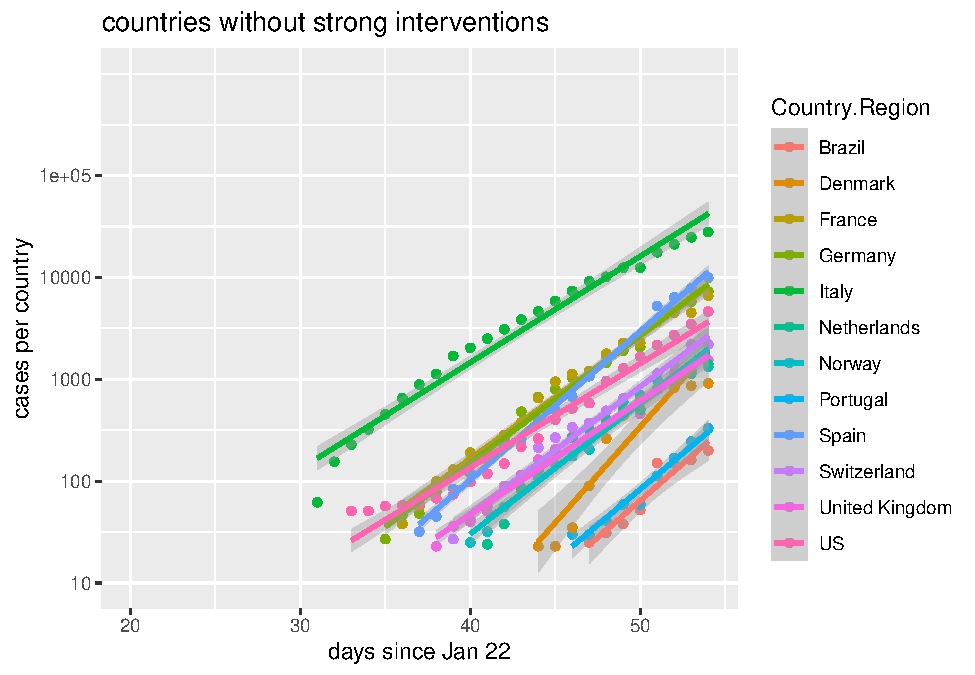
\includegraphics{PlotData_files/figure-latex/plotNIcountries-1.pdf}

Countries that seemed to have early strong intervention plans. This list
is somewhat arbitrary, but these can be more clearly visualized on their
own in any case.

\begin{Shaded}
\begin{Highlighting}[]
\KeywordTok{ggplot}\NormalTok{(}\DataTypeTok{data=}\KeywordTok{filter}\NormalTok{(confirmed_long2,Country.Region}\OperatorTok{==}\StringTok{"China"} \OperatorTok{|}\NormalTok{Country.Region}\OperatorTok{==}\StringTok{"Korea, South"} \OperatorTok{|}\NormalTok{Country.Region}\OperatorTok{==}\StringTok{"Japan"} \OperatorTok{|}\StringTok{ }\NormalTok{Country.Region}\OperatorTok{==}\StringTok{"Singapore"} \OperatorTok{|}\NormalTok{Country.Region}\OperatorTok{==}\StringTok{"Taiwan*"}\NormalTok{    ,cases}\OperatorTok{>}\DecValTok{20}\NormalTok{) , }\KeywordTok{aes}\NormalTok{(}\DataTypeTok{x=}\NormalTok{delta.days,}\DataTypeTok{y=}\KeywordTok{log}\NormalTok{(cases,}\DataTypeTok{base=}\DecValTok{10}\NormalTok{) ,}\DataTypeTok{color=}\NormalTok{ Country.Region , }\DataTypeTok{group=}\NormalTok{Country.Region)) }\OperatorTok{+}
\StringTok{  }\KeywordTok{geom_point}\NormalTok{(}\KeywordTok{aes}\NormalTok{(}\DataTypeTok{color=}\NormalTok{ Country.Region))}\OperatorTok{+}
\StringTok{    }\KeywordTok{geom_smooth}\NormalTok{(}\DataTypeTok{method =} \StringTok{"loess"}\NormalTok{,}\DataTypeTok{formula =}\NormalTok{ y }\OperatorTok{~}\StringTok{ }\NormalTok{x) }\OperatorTok{+}\StringTok{ }
\StringTok{  }\KeywordTok{scale_y_continuous}\NormalTok{( }\DataTypeTok{limits=}\KeywordTok{c}\NormalTok{(}\DecValTok{1}\NormalTok{,}\DecValTok{6}\NormalTok{),}\DataTypeTok{breaks=}\KeywordTok{c}\NormalTok{(}\DecValTok{1}\NormalTok{,}\DecValTok{2}\NormalTok{,}\DecValTok{3}\NormalTok{,}\DecValTok{4}\NormalTok{,}\DecValTok{5}\NormalTok{), }\DataTypeTok{labels=}\KeywordTok{c}\NormalTok{(}\DecValTok{10}\NormalTok{,}\DecValTok{100}\NormalTok{,}\DecValTok{1000}\NormalTok{,}\DecValTok{10000}\NormalTok{,}\DecValTok{100000}\NormalTok{))}\OperatorTok{+}
\StringTok{   }\KeywordTok{scale_x_continuous}\NormalTok{( }\DataTypeTok{limits=}\KeywordTok{c}\NormalTok{(}\DecValTok{20}\NormalTok{,}\DecValTok{54}\NormalTok{))}\OperatorTok{+}
\StringTok{  }\KeywordTok{labs}\NormalTok{( }\DataTypeTok{x=}\StringTok{"days since Jan 22"}\NormalTok{ , }\DataTypeTok{y=}\StringTok{"cases per country"}\NormalTok{ , }\DataTypeTok{title=}\StringTok{"countries with interventions"}\NormalTok{)}
\end{Highlighting}
\end{Shaded}

\begin{verbatim}
## Warning: Removed 39 rows containing non-finite values (stat_smooth).
\end{verbatim}

\begin{verbatim}
## Warning: Removed 39 rows containing missing values (geom_point).
\end{verbatim}

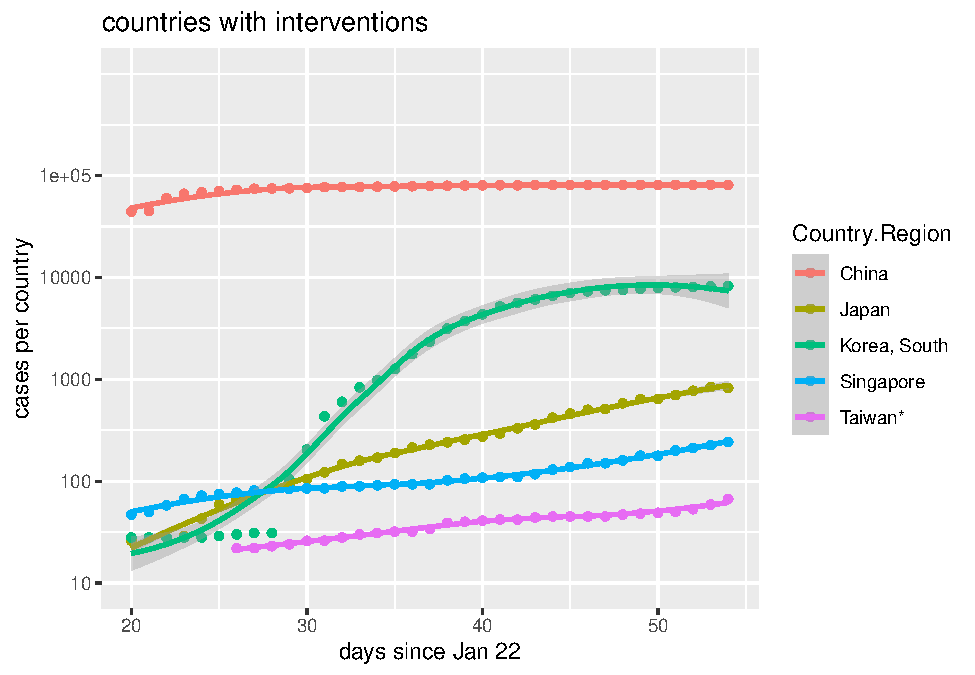
\includegraphics{PlotData_files/figure-latex/plotICountries-1.pdf}

South American countries: Leave the date-range the same so that slopes
can be visually compared.

\begin{Shaded}
\begin{Highlighting}[]
\KeywordTok{ggplot}\NormalTok{(}\DataTypeTok{data=}\KeywordTok{filter}\NormalTok{(confirmed_long2,Country.Region}\OperatorTok{==}\StringTok{"Brazil"} \OperatorTok{|}\NormalTok{Country.Region}\OperatorTok{==}\StringTok{"Argentina"} \OperatorTok{|}\NormalTok{Country.Region}\OperatorTok{==}\StringTok{"Chile"} \OperatorTok{|}\StringTok{ }\NormalTok{Country.Region}\OperatorTok{==}\StringTok{"Mexico"} \OperatorTok{|}\NormalTok{Country.Region}\OperatorTok{==}\StringTok{"Peru"}\NormalTok{    ,cases}\OperatorTok{>}\DecValTok{20}\NormalTok{) , }\KeywordTok{aes}\NormalTok{(}\DataTypeTok{x=}\NormalTok{delta.days,}\DataTypeTok{y=}\KeywordTok{log}\NormalTok{(cases,}\DataTypeTok{base=}\DecValTok{10}\NormalTok{) ,}\DataTypeTok{color=}\NormalTok{ Country.Region , }\DataTypeTok{group=}\NormalTok{Country.Region)) }\OperatorTok{+}
\StringTok{  }\KeywordTok{geom_point}\NormalTok{(}\KeywordTok{aes}\NormalTok{(}\DataTypeTok{color=}\NormalTok{ Country.Region))}\OperatorTok{+}
\StringTok{    }\KeywordTok{geom_smooth}\NormalTok{(}\DataTypeTok{method =} \StringTok{"lm"}\NormalTok{, }\DataTypeTok{formula =}\NormalTok{ y }\OperatorTok{~}\StringTok{ }\NormalTok{x) }\OperatorTok{+}\StringTok{ }
\StringTok{  }\KeywordTok{scale_y_continuous}\NormalTok{( }\DataTypeTok{limits=}\KeywordTok{c}\NormalTok{(}\DecValTok{1}\NormalTok{,}\DecValTok{6}\NormalTok{),}\DataTypeTok{breaks=}\KeywordTok{c}\NormalTok{(}\DecValTok{1}\NormalTok{,}\DecValTok{2}\NormalTok{,}\DecValTok{3}\NormalTok{,}\DecValTok{4}\NormalTok{,}\DecValTok{5}\NormalTok{), }\DataTypeTok{labels=}\KeywordTok{c}\NormalTok{(}\DecValTok{10}\NormalTok{,}\DecValTok{100}\NormalTok{,}\DecValTok{1000}\NormalTok{,}\DecValTok{10000}\NormalTok{,}\DecValTok{100000}\NormalTok{))}\OperatorTok{+}
\StringTok{  }\KeywordTok{scale_x_continuous}\NormalTok{( }\DataTypeTok{limits=}\KeywordTok{c}\NormalTok{(}\DecValTok{20}\NormalTok{,}\DecValTok{54}\NormalTok{))}\OperatorTok{+}
\StringTok{  }\KeywordTok{labs}\NormalTok{( }\DataTypeTok{x=}\StringTok{"days since Jan 22"}\NormalTok{ , }\DataTypeTok{y=}\StringTok{"cases per country"}\NormalTok{, }\DataTypeTok{title=}\StringTok{"South American countries"}\NormalTok{)}
\end{Highlighting}
\end{Shaded}

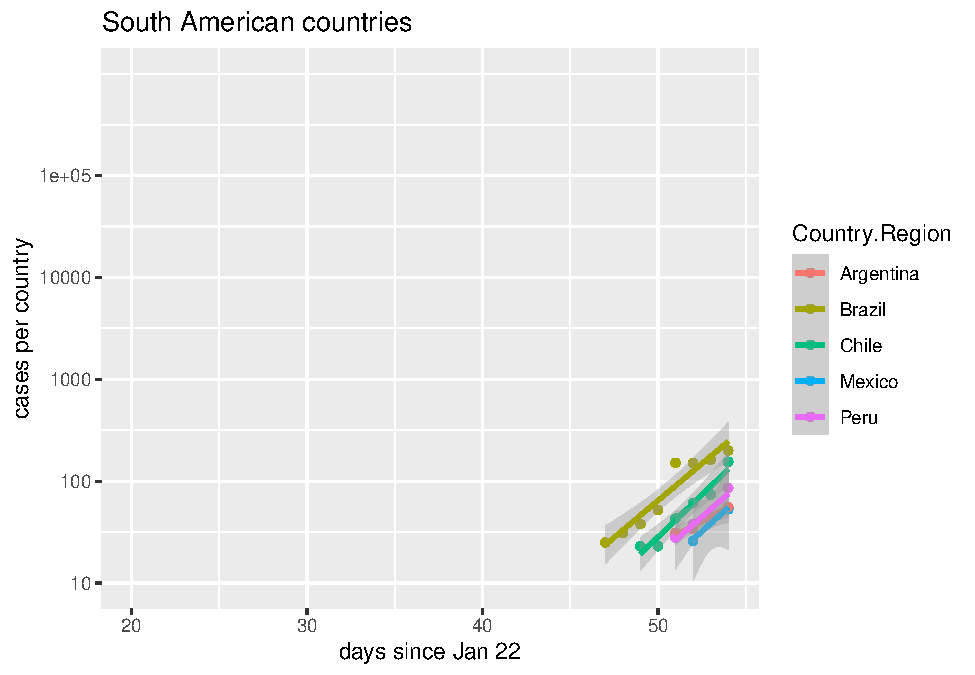
\includegraphics{PlotData_files/figure-latex/plotSACountries-1.pdf}

Plot Canada.

\begin{Shaded}
\begin{Highlighting}[]
\CommentTok{#Canadians}
\KeywordTok{ggplot}\NormalTok{(}\DataTypeTok{data=}\KeywordTok{filter}\NormalTok{(confirmed_long2, Country.Region}\OperatorTok{==}\StringTok{"Canada"}\NormalTok{   ,cases}\OperatorTok{>}\DecValTok{20}\NormalTok{) , }\KeywordTok{aes}\NormalTok{(}\DataTypeTok{x=}\NormalTok{delta.days,}\DataTypeTok{y=}\KeywordTok{log}\NormalTok{(cases,}\DataTypeTok{base=}\DecValTok{10}\NormalTok{) ,}\DataTypeTok{color=}\NormalTok{ Province.State , }\DataTypeTok{group=}\NormalTok{Province.State)) }\OperatorTok{+}
\StringTok{  }\KeywordTok{geom_point}\NormalTok{(}\KeywordTok{aes}\NormalTok{(}\DataTypeTok{color=}\NormalTok{ Province.State))}\OperatorTok{+}
\StringTok{    }\KeywordTok{geom_smooth}\NormalTok{(}\DataTypeTok{method =} \StringTok{"lm"}\NormalTok{, }\DataTypeTok{formula =}\NormalTok{ y }\OperatorTok{~}\StringTok{ }\NormalTok{x) }\OperatorTok{+}\StringTok{ }
\StringTok{  }\KeywordTok{scale_y_continuous}\NormalTok{( }\DataTypeTok{limits=}\KeywordTok{c}\NormalTok{(}\DecValTok{1}\NormalTok{,}\DecValTok{6}\NormalTok{),}\DataTypeTok{breaks=}\KeywordTok{c}\NormalTok{(}\DecValTok{1}\NormalTok{,}\DecValTok{2}\NormalTok{,}\DecValTok{3}\NormalTok{,}\DecValTok{4}\NormalTok{,}\DecValTok{5}\NormalTok{), }\DataTypeTok{labels=}\KeywordTok{c}\NormalTok{(}\DecValTok{10}\NormalTok{,}\DecValTok{100}\NormalTok{,}\DecValTok{1000}\NormalTok{,}\DecValTok{10000}\NormalTok{,}\DecValTok{100000}\NormalTok{))}\OperatorTok{+}
\StringTok{  }\KeywordTok{scale_x_continuous}\NormalTok{( }\DataTypeTok{limits=}\KeywordTok{c}\NormalTok{(}\DecValTok{20}\NormalTok{,}\DecValTok{54}\NormalTok{))}\OperatorTok{+}
\StringTok{  }\KeywordTok{labs}\NormalTok{( }\DataTypeTok{x=}\StringTok{"days since Jan 22"}\NormalTok{ , }\DataTypeTok{y=}\StringTok{"cases per country"}\NormalTok{, }\DataTypeTok{title=}\StringTok{"Canadian states*"}\NormalTok{)}
\end{Highlighting}
\end{Shaded}

\begin{verbatim}
## Warning in qt((1 - level)/2, df): NaNs produced
\end{verbatim}

\begin{verbatim}
## Warning in max(ids, na.rm = TRUE): no non-missing arguments to max;
## returning -Inf
\end{verbatim}

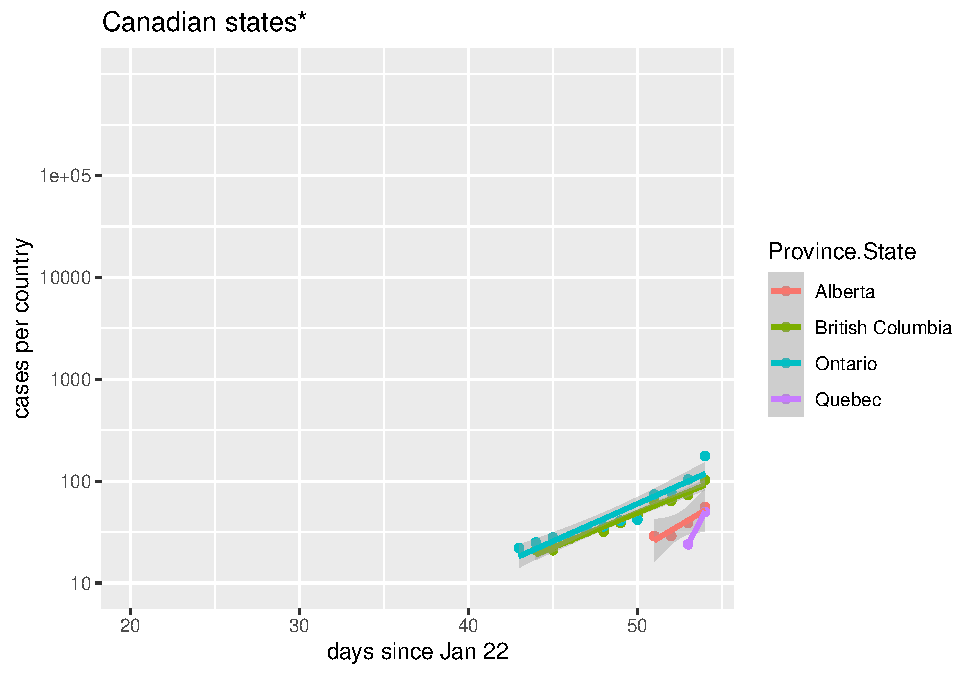
\includegraphics{PlotData_files/figure-latex/PlotCanadianProvinces-1.pdf}

\#Do Bayesian fitting of subsets of the data

This is a very un-sophisiticated method. Just assume that the number of
cases on day t+1 is Poisson distributed with lambda = (cases on day t )
* lambda\_1 where lambda\_1 is the per case number of new infections.
One thing to think about is that the cases are all supposedly taken out
of circulation, so they cannot be literally infecting people on the next
day, although they could have infected them before and not been
detected. I think a more plausible interpretation of the model is that
there are many undetected cases, of which a fraction are detected. If
the fraction detected is relatively constant, then the dynamics of the
detected cases match those of the undetected cases.

It would be great to build a more complex model including: 1. testing
rates and probabilty of being tested given infected, i.e.~to build a
model of how the medical professionals choose who to test. 2. day of the
week effects on testing rate 3. the incubation period 4. variance in the
infection rate due to un-measured environmental variance

This writes the stan file. If you have the stan file already can leave
this unevaluated

\begin{Shaded}
\begin{Highlighting}[]
\KeywordTok{sink}\NormalTok{(}\StringTok{"model_PoissonOnly.stan"}\NormalTok{)}
\KeywordTok{cat}\NormalTok{(}\StringTok{"}

\StringTok{    data \{}
\StringTok{    int<lower=0> n; // number of time points}
\StringTok{    int days[n];}
\StringTok{    int total_cases[n] ;}
\StringTok{    \}}
\StringTok{    transformed data\{}
\StringTok{    int new_cases[n] ; //really only need n-1 but keep the indexing the same for simplicity}
\StringTok{    new_cases[1]=0;}
\StringTok{    for(i in 2:n)\{}
\StringTok{    new_cases[i]=total_cases[i]-total_cases[i-1];}
\StringTok{    \}}
\StringTok{    \}}
\StringTok{    parameters \{}
\StringTok{    real <lower=0 , upper=50.0> lambda ; // Poisson parameter for the growth rate}
\StringTok{    \}}
\StringTok{    model \{}
\StringTok{    for(i in 2:n)\{}
\StringTok{    new_cases[i] ~ poisson(total_cases[i-1]*lambda); // update for each time step is the sum of Poisson RVs with mean lambda}
\StringTok{    \}}
\StringTok{    \}}
\StringTok{    }
\StringTok{      }
\StringTok{    }
\StringTok{    "}\NormalTok{,}\DataTypeTok{fill =} \OtherTok{TRUE}\NormalTok{)}
\KeywordTok{sink}\NormalTok{()}
\end{Highlighting}
\end{Shaded}

Note that the only parameter being fit is lambda, which is the per case
Poisson parameter. Thus the daily multiplication factor is this lambda,
and so the doubling time is log(2)/(log(1+lambda))

US growth rate inference

\begin{Shaded}
\begin{Highlighting}[]
\KeywordTok{print}\NormalTok{(fit_poiss, }\DataTypeTok{pars=}\KeywordTok{c}\NormalTok{(}\StringTok{"lambda"}\NormalTok{),}\DataTypeTok{digits_summary =} \DecValTok{3}\NormalTok{)}
\end{Highlighting}
\end{Shaded}

\begin{verbatim}
## Inference for Stan model: model_PoissonOnly.
## 4 chains, each with iter=1000; warmup=500; thin=1; 
## post-warmup draws per chain=500, total post-warmup draws=2000.
## 
##         mean se_mean    sd  2.5%   25%   50%   75% 97.5% n_eff  Rhat
## lambda 0.304       0 0.005 0.295 0.301 0.304 0.307 0.313   590 1.007
## 
## Samples were drawn using NUTS(diag_e) at Mon Mar 16 22:19:41 2020.
## For each parameter, n_eff is a crude measure of effective sample size,
## and Rhat is the potential scale reduction factor on split chains (at 
## convergence, Rhat=1).
\end{verbatim}

For California

\begin{Shaded}
\begin{Highlighting}[]
\KeywordTok{print}\NormalTok{(fit_poiss, }\DataTypeTok{pars=}\KeywordTok{c}\NormalTok{(}\StringTok{"lambda"}\NormalTok{),}\DataTypeTok{digits_summary =} \DecValTok{3}\NormalTok{)}
\end{Highlighting}
\end{Shaded}

\begin{verbatim}
## Inference for Stan model: model_PoissonOnly.
## 4 chains, each with iter=1000; warmup=500; thin=1; 
## post-warmup draws per chain=500, total post-warmup draws=2000.
## 
##         mean se_mean    sd  2.5%   25%   50%   75% 97.5% n_eff  Rhat
## lambda 0.261   0.001 0.012 0.239 0.253 0.261 0.268 0.284   530 1.003
## 
## Samples were drawn using NUTS(diag_e) at Mon Mar 16 22:19:42 2020.
## For each parameter, n_eff is a crude measure of effective sample size,
## and Rhat is the potential scale reduction factor on split chains (at 
## convergence, Rhat=1).
\end{verbatim}

For New York

\begin{Shaded}
\begin{Highlighting}[]
\KeywordTok{print}\NormalTok{(fit_poiss, }\DataTypeTok{pars=}\KeywordTok{c}\NormalTok{(}\StringTok{"lambda"}\NormalTok{),}\DataTypeTok{digits_summary =} \DecValTok{3}\NormalTok{)}
\end{Highlighting}
\end{Shaded}

\begin{verbatim}
## Inference for Stan model: model_PoissonOnly.
## 4 chains, each with iter=1000; warmup=500; thin=1; 
## post-warmup draws per chain=500, total post-warmup draws=2000.
## 
##         mean se_mean    sd 2.5%   25%  50%   75% 97.5% n_eff  Rhat
## lambda 0.341       0 0.011 0.32 0.333 0.34 0.348 0.362   894 1.002
## 
## Samples were drawn using NUTS(diag_e) at Mon Mar 16 22:19:43 2020.
## For each parameter, n_eff is a crude measure of effective sample size,
## and Rhat is the potential scale reduction factor on split chains (at 
## convergence, Rhat=1).
\end{verbatim}

Italy

\begin{Shaded}
\begin{Highlighting}[]
\KeywordTok{print}\NormalTok{(fit_poiss, }\DataTypeTok{pars=}\KeywordTok{c}\NormalTok{(}\StringTok{"lambda"}\NormalTok{),}\DataTypeTok{digits_summary =} \DecValTok{3}\NormalTok{)}
\end{Highlighting}
\end{Shaded}

\begin{verbatim}
## Inference for Stan model: model_PoissonOnly.
## 4 chains, each with iter=1000; warmup=500; thin=1; 
## post-warmup draws per chain=500, total post-warmup draws=2000.
## 
##         mean se_mean    sd  2.5%   25%   50%   75% 97.5% n_eff  Rhat
## lambda 0.196       0 0.001 0.193 0.195 0.196 0.196 0.198   797 1.001
## 
## Samples were drawn using NUTS(diag_e) at Mon Mar 16 22:19:45 2020.
## For each parameter, n_eff is a crude measure of effective sample size,
## and Rhat is the potential scale reduction factor on split chains (at 
## convergence, Rhat=1).
\end{verbatim}

France

\begin{Shaded}
\begin{Highlighting}[]
\KeywordTok{print}\NormalTok{(fit_poiss, }\DataTypeTok{pars=}\KeywordTok{c}\NormalTok{(}\StringTok{"lambda"}\NormalTok{),}\DataTypeTok{digits_summary =} \DecValTok{3}\NormalTok{)}
\end{Highlighting}
\end{Shaded}

\begin{verbatim}
## Inference for Stan model: model_PoissonOnly.
## 4 chains, each with iter=1000; warmup=500; thin=1; 
## post-warmup draws per chain=500, total post-warmup draws=2000.
## 
##         mean se_mean    sd  2.5%   25%   50%   75% 97.5% n_eff  Rhat
## lambda 0.272       0 0.003 0.265 0.269 0.272 0.274 0.278   676 1.003
## 
## Samples were drawn using NUTS(diag_e) at Mon Mar 16 22:19:45 2020.
## For each parameter, n_eff is a crude measure of effective sample size,
## and Rhat is the potential scale reduction factor on split chains (at 
## convergence, Rhat=1).
\end{verbatim}

Brazil

\begin{Shaded}
\begin{Highlighting}[]
\KeywordTok{print}\NormalTok{(fit_poiss, }\DataTypeTok{pars=}\KeywordTok{c}\NormalTok{(}\StringTok{"lambda"}\NormalTok{),}\DataTypeTok{digits_summary =} \DecValTok{3}\NormalTok{)}
\end{Highlighting}
\end{Shaded}

\begin{verbatim}
## Inference for Stan model: model_PoissonOnly.
## 4 chains, each with iter=1000; warmup=500; thin=1; 
## post-warmup draws per chain=500, total post-warmup draws=2000.
## 
##         mean se_mean    sd  2.5%   25%   50%   75% 97.5% n_eff  Rhat
## lambda 0.288   0.001 0.021 0.247 0.273 0.288 0.302  0.33   664 1.002
## 
## Samples were drawn using NUTS(diag_e) at Mon Mar 16 22:19:46 2020.
## For each parameter, n_eff is a crude measure of effective sample size,
## and Rhat is the potential scale reduction factor on split chains (at 
## convergence, Rhat=1).
\end{verbatim}

And for the Canadians

\begin{Shaded}
\begin{Highlighting}[]
\NormalTok{mydata.sub <-}\StringTok{ }\KeywordTok{filter}\NormalTok{(confirmed_long2,cases}\OperatorTok{>}\DecValTok{20}\NormalTok{,Province.State }\OperatorTok{==}\StringTok{ "Ontario"}\NormalTok{)  }

\NormalTok{mindays=}\KeywordTok{min}\NormalTok{(mydata.sub}\OperatorTok{$}\NormalTok{delta.days)}


\NormalTok{mydata.sub <-}\StringTok{ }\KeywordTok{mutate}\NormalTok{(mydata.sub,}\DataTypeTok{days=}\NormalTok{delta.days}\OperatorTok{-}\NormalTok{mindays) }\OperatorTok\StringTok{ }\KeywordTok{arrange}\NormalTok{(days)   }\OperatorTok
\StringTok{  }\KeywordTok{rename}\NormalTok{(}\DataTypeTok{total_cases=}\NormalTok{cases)}

\NormalTok{n=}\KeywordTok{max}\NormalTok{(mydata.sub}\OperatorTok{$}\NormalTok{days)}\OperatorTok{+}\DecValTok{1}


\NormalTok{stan_data <-}\StringTok{ }\KeywordTok{c}\NormalTok{(mydata.sub[}\KeywordTok{c}\NormalTok{(}\StringTok{"days"}\NormalTok{,}\StringTok{"total_cases"}\NormalTok{)], }\KeywordTok{list}\NormalTok{(}\DataTypeTok{n=}\NormalTok{n)) }

\CommentTok{#fit the model}
\NormalTok{fit_poiss <-}\StringTok{ }\KeywordTok{stan}\NormalTok{(}\DataTypeTok{file =} \StringTok{'model_PoissonOnly.stan'}\NormalTok{, }
                \DataTypeTok{data =}\NormalTok{stan_data, }\DataTypeTok{chains =} \DecValTok{4}\NormalTok{,}\DataTypeTok{iter =} \DecValTok{1000}\NormalTok{, }\DataTypeTok{seed =} \DecValTok{2131231}\NormalTok{ )}
\end{Highlighting}
\end{Shaded}

\begin{Shaded}
\begin{Highlighting}[]
\KeywordTok{print}\NormalTok{(fit_poiss, }\DataTypeTok{pars=}\KeywordTok{c}\NormalTok{(}\StringTok{"lambda"}\NormalTok{),}\DataTypeTok{digits_summary =} \DecValTok{3}\NormalTok{)}
\end{Highlighting}
\end{Shaded}

\begin{verbatim}
## Inference for Stan model: model_PoissonOnly.
## 4 chains, each with iter=1000; warmup=500; thin=1; 
## post-warmup draws per chain=500, total post-warmup draws=2000.
## 
##         mean se_mean    sd  2.5%   25%   50%   75% 97.5% n_eff  Rhat
## lambda 0.288   0.001 0.021 0.247 0.273 0.288 0.302  0.33   664 1.002
## 
## Samples were drawn using NUTS(diag_e) at Mon Mar 16 22:19:46 2020.
## For each parameter, n_eff is a crude measure of effective sample size,
## and Rhat is the potential scale reduction factor on split chains (at 
## convergence, Rhat=1).
\end{verbatim}

\begin{Shaded}
\begin{Highlighting}[]
\NormalTok{mydata.sub <-}\StringTok{ }\KeywordTok{filter}\NormalTok{(confirmed_long2,cases}\OperatorTok{>}\DecValTok{20}\NormalTok{,Province.State }\OperatorTok{==}\StringTok{ "British Columbia"}\NormalTok{)  }

\NormalTok{mindays=}\KeywordTok{min}\NormalTok{(mydata.sub}\OperatorTok{$}\NormalTok{delta.days)}


\NormalTok{mydata.sub <-}\StringTok{ }\KeywordTok{mutate}\NormalTok{(mydata.sub,}\DataTypeTok{days=}\NormalTok{delta.days}\OperatorTok{-}\NormalTok{mindays) }\OperatorTok\StringTok{ }\KeywordTok{arrange}\NormalTok{(days)   }\OperatorTok
\StringTok{  }\KeywordTok{rename}\NormalTok{(}\DataTypeTok{total_cases=}\NormalTok{cases)}

\NormalTok{n=}\KeywordTok{max}\NormalTok{(mydata.sub}\OperatorTok{$}\NormalTok{days)}\OperatorTok{+}\DecValTok{1}


\NormalTok{stan_data <-}\StringTok{ }\KeywordTok{c}\NormalTok{(mydata.sub[}\KeywordTok{c}\NormalTok{(}\StringTok{"days"}\NormalTok{,}\StringTok{"total_cases"}\NormalTok{)], }\KeywordTok{list}\NormalTok{(}\DataTypeTok{n=}\NormalTok{n)) }

\CommentTok{#fit the model}
\NormalTok{fit_poiss <-}\StringTok{ }\KeywordTok{stan}\NormalTok{(}\DataTypeTok{file =} \StringTok{'model_PoissonOnly.stan'}\NormalTok{, }
                \DataTypeTok{data =}\NormalTok{stan_data, }\DataTypeTok{chains =} \DecValTok{4}\NormalTok{,}\DataTypeTok{iter =} \DecValTok{1000}\NormalTok{, }\DataTypeTok{seed =} \DecValTok{2131231}\NormalTok{ )}
\end{Highlighting}
\end{Shaded}

\begin{Shaded}
\begin{Highlighting}[]
\KeywordTok{print}\NormalTok{(fit_poiss, }\DataTypeTok{pars=}\KeywordTok{c}\NormalTok{(}\StringTok{"lambda"}\NormalTok{),}\DataTypeTok{digits_summary =} \DecValTok{3}\NormalTok{)}
\end{Highlighting}
\end{Shaded}

\begin{verbatim}
## Inference for Stan model: model_PoissonOnly.
## 4 chains, each with iter=1000; warmup=500; thin=1; 
## post-warmup draws per chain=500, total post-warmup draws=2000.
## 
##         mean se_mean    sd  2.5%   25%   50%   75% 97.5% n_eff  Rhat
## lambda 0.288   0.001 0.021 0.247 0.273 0.288 0.302  0.33   664 1.002
## 
## Samples were drawn using NUTS(diag_e) at Mon Mar 16 22:19:46 2020.
## For each parameter, n_eff is a crude measure of effective sample size,
## and Rhat is the potential scale reduction factor on split chains (at 
## convergence, Rhat=1).
\end{verbatim}

\begin{Shaded}
\begin{Highlighting}[]
\NormalTok{mydata.sub <-}\StringTok{ }\KeywordTok{filter}\NormalTok{(confirmed_long2,cases}\OperatorTok{>}\DecValTok{20}\NormalTok{,Province.State }\OperatorTok{==}\StringTok{ "Alberta"}\NormalTok{)  }

\NormalTok{mindays=}\KeywordTok{min}\NormalTok{(mydata.sub}\OperatorTok{$}\NormalTok{delta.days)}


\NormalTok{mydata.sub <-}\StringTok{ }\KeywordTok{mutate}\NormalTok{(mydata.sub,}\DataTypeTok{days=}\NormalTok{delta.days}\OperatorTok{-}\NormalTok{mindays) }\OperatorTok\StringTok{ }\KeywordTok{arrange}\NormalTok{(days)   }\OperatorTok
\StringTok{  }\KeywordTok{rename}\NormalTok{(}\DataTypeTok{total_cases=}\NormalTok{cases)}

\NormalTok{n=}\KeywordTok{max}\NormalTok{(mydata.sub}\OperatorTok{$}\NormalTok{days)}\OperatorTok{+}\DecValTok{1}


\NormalTok{stan_data <-}\StringTok{ }\KeywordTok{c}\NormalTok{(mydata.sub[}\KeywordTok{c}\NormalTok{(}\StringTok{"days"}\NormalTok{,}\StringTok{"total_cases"}\NormalTok{)], }\KeywordTok{list}\NormalTok{(}\DataTypeTok{n=}\NormalTok{n)) }

\CommentTok{#fit the model}
\NormalTok{fit_poiss <-}\StringTok{ }\KeywordTok{stan}\NormalTok{(}\DataTypeTok{file =} \StringTok{'model_PoissonOnly.stan'}\NormalTok{, }
                \DataTypeTok{data =}\NormalTok{stan_data, }\DataTypeTok{chains =} \DecValTok{4}\NormalTok{,}\DataTypeTok{iter =} \DecValTok{1000}\NormalTok{, }\DataTypeTok{seed =} \DecValTok{2131231}\NormalTok{ )}
\end{Highlighting}
\end{Shaded}

\begin{Shaded}
\begin{Highlighting}[]
\KeywordTok{print}\NormalTok{(fit_poiss, }\DataTypeTok{pars=}\KeywordTok{c}\NormalTok{(}\StringTok{"lambda"}\NormalTok{),}\DataTypeTok{digits_summary =} \DecValTok{3}\NormalTok{)}
\end{Highlighting}
\end{Shaded}

\begin{verbatim}
## Inference for Stan model: model_PoissonOnly.
## 4 chains, each with iter=1000; warmup=500; thin=1; 
## post-warmup draws per chain=500, total post-warmup draws=2000.
## 
##         mean se_mean    sd  2.5%   25%   50%   75% 97.5% n_eff  Rhat
## lambda 0.288   0.001 0.021 0.247 0.273 0.288 0.302  0.33   664 1.002
## 
## Samples were drawn using NUTS(diag_e) at Mon Mar 16 22:19:46 2020.
## For each parameter, n_eff is a crude measure of effective sample size,
## and Rhat is the potential scale reduction factor on split chains (at 
## convergence, Rhat=1).
\end{verbatim}


\end{document}
